\subsubsection{Prototype Development with separate databases}
Developing the prototype began with creating the Catalogue Microservice first. This appeared to be a good place to start: create a basic MVC (Model-View-Controller) front-end that would connect to the Catalogue Microservice to display the list of items in the catalogue. Initially the idea was to create the Databases, with a table with data, connect to the microservice and then, through the API Gateway, connect with the front-end. Through research, it was deemed this was a difficult task to do. 

The API Gateway itself being a implemented using JSON documents and using a middle-ware technology, such as Ocelot Insert Citation, to implement. This would need further researching purely for this section of the prototype.

Instead, creating a blank Database was decided upon. From here, connect it to the API for the microservice and then to the front-end. The API Gateway has been omitted, at this stage, purely as there is only one API and to see the system working, albeit in a very basic way. Future, successful additions of microservices will see the API Gateway being added. 

NOTE: Docker support was added to begin with, but proved to be difficult to work with. Instead, the prototype was developed without Docker support. Which will be added later, after further researching and small prototype builds to use the features needed for this project. This decision was taken as it was necessary to provide a working prototype of the proposed system within the time-frame than being delayed by understanding and then fixing the problem incurred using Docker. If docker is not able to be added to the prototype. Then this will be documented in the evaluation section and discussed as fully as possible.

\subsubsection{Catalogue Microservice}
Creating the database was relatively simple: creating an account with Azure and creating the database and the server for its use. From here, the connection information needed is provided by Azure. Conveniently providing string connections depending on the type of connection wanted. ADO.NET was chosen. All that would be needed is having the string connection copy and pasted into the Appsettings.JSON file of the Catalogue Microservice. By adding the string to this file, enables Visual Studio to locate and connect to the server successfully to begin Entity Framework coding for manipulation/interrogation of the database.
\begin{figure}[h]
	\caption{Azure ADO.NET Connection String for the server containing the Catalogue Microservice Database}
	\label{fig:AzureCataMSImage}
	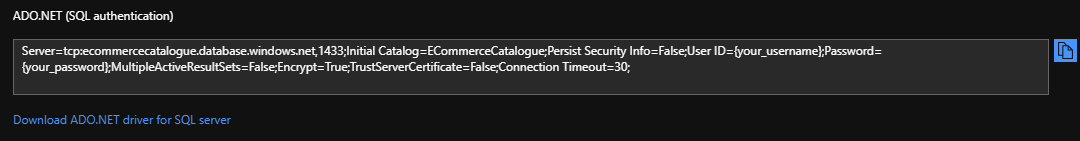
\includegraphics[height=3cm, width=20cm]{/DevelopmentPics/AzureCatalogueMSImage}
\end{figure}
\pagebreak
\begin{figure}[h]
	\caption{Visual Studio Appsetting.JSON connection string. Partial View}
	\label{fig:VSPartialCataMSImage}
	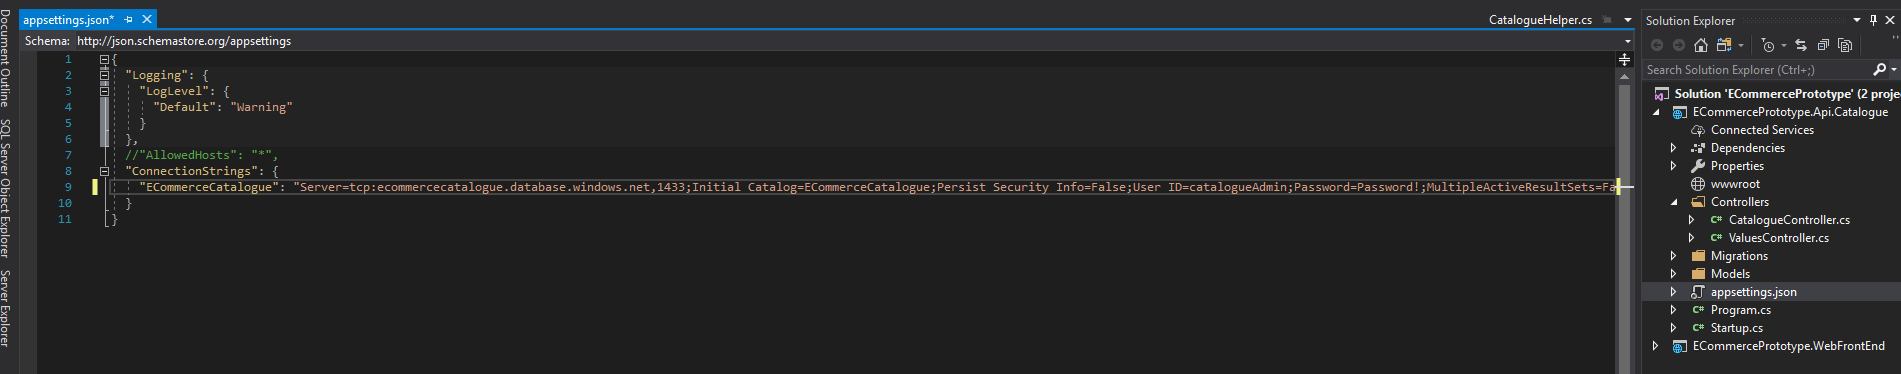
\includegraphics[height=5cm, width=15cm]{/DevelopmentPics/VSConnectionStringCatalogueMSImage}
\end{figure}

Using the Microsoft.Docs website, specifically the Entity Framework (EF) section, is very useful to gain an understanding, with example tutorials provided on how to use this feature for Database Manipulation \cite{EFMicrosoft}, \cite{EFMicrosoftQuickStart}. Also, an interesting blog on the c-sharpcorner website on this \cite{EFCSharpCorner}. And this blog (INSERT CITATION)

After reading over these sites. The project was started. Developing the Catalogue API first. Connection string and Entity framework were first to be created and inserted. Creating a DBContext class for the system to interact with the Catalogue database. This class inherits from the DBContext class that enables a session created with the databases, getting the connection string through the Appsettings.JSON file, and allows for querying and saving entities to the database. 

The Catalogue class was created using the system.ComponentModel.DataAnnotations.Schema to enable the properties to be used to create columns within the created table, within the CatalogueDB, that would store all catalogue item records. This was done by using Entity frameworks migration function to create the table based on the structure of the class and then updating the database with this migration. This was done successfully. Proving the system was connected to this database, through the Azure server, successfully. Of note, the Property storing the location of the picture for the item was not created at this point. It was done later.
 
Based on research (INSERT CITATION) it was deemed necessary to provide an interface that would provide the methods needed, for this microservice, to query the database. Specifically Getall() and Get(int id) methods. From here, the CatalogueManager class was created, that inherits from this interface. To provide implementation of these methods. The CatalogueManager class creates a read-only only object of the CatalogueDbContext that it uses to perform the methods upon. Returning the required entities - either a full list of all Catalogue Items or a single item based on its id in the database. 

To enable this database connection to be used repeatedly, the DBContext, Data Repository interface and data manager class needed dependency injection by adding them as services to the ConfigurstionServices method of startup class \cite{DependInjectMicrosoft}. BY setting the data repository \& catalogue manager as both scoped and transient, ensures each interaction with the database is created each time its requested and only once per request. Preventing duplication of requests within the one request.
\begin{figure}[h]
	\caption{Visual Studio Dependency Injection for the Catalogue Microservice}
	\label{fig:VSDICataMs}
	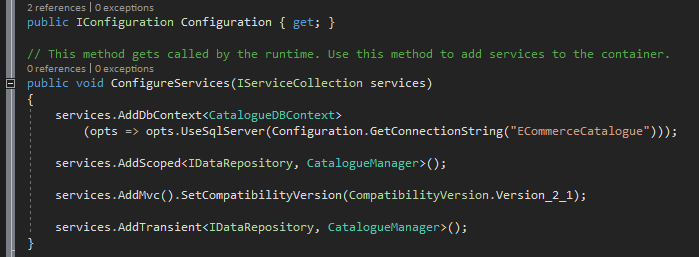
\includegraphics[height=6.5cm, width=15cm]{/DevelopmentPics/VSDICataMSImage}
\end{figure}

The final part of the Catalogue microservice to complete was the API Controller. This controller would be controlling how the database is interacted with, using HTTP Verbs, to expose what the front-end website can consume from this microservice. As the controller will be using a read-only object of the IDataRepository class, the only verbs being exposed will be Getall() and get() a single catalogue item by its id in the database.
\begin{figure}[h]
	\caption{Visual Studio API Controller for Catalogue Microservice}
	\label{fig:VSAPiCataMs}
	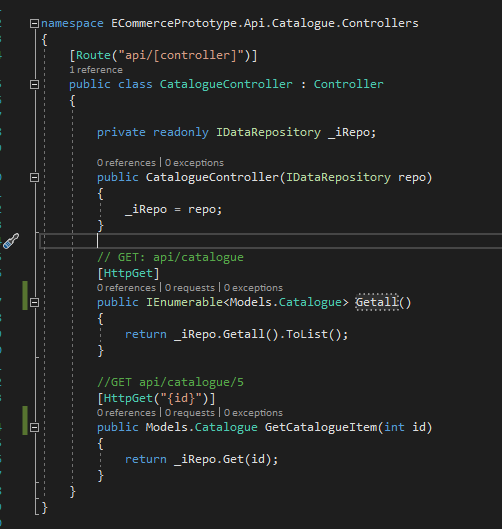
\includegraphics[height=12cm, width=11cm]{/DevelopmentPics/VSCataAPIController}
\end{figure}
Microsoft SQL server management system was used to connect to the database, trough its server, to insert several records to display on the website. After the inserts created, they were checked within the Azure portal dashboard to see they were present.

The Microservice was also run, as an API on the localhost, to display all the records created. And that a single record can be viewed by passing in an id to the URL.

(INSERT PICS??)

\subsubsection{Basket Microservice}

NOTE: All API's will be created using the same design of a DBContext, IDataRepository and Manager interfaces/classes. Only differences being naming convention and CRUD implementation. Which will be identified for each API.
\subsubsection{Prototype Development with a single centralised database}
\subsubsection{Front-End website development}
The website will be developed using the MVC architecture pattern. The Views applicable to each Microservice will be separated, as the standard when developing web applications using .NET Core, using folders. Each folder named after the corresponding controller that controls each group of Views.
To emphasise the use of Agile throughout the development cycle, the website will be developed upon after each Microservice has been successfully implemented. The different sections being developed are discussed:
\paragraph{Displaying Catalogue Items}
This section of the prototype was created with the MVC template provided by Microsoft as the basis. The implemented code was replaced with the required code for views and controllers.
Firstly, the models needed were created. A copy of the catalogue class from the Catalogue Microservice was created, as this would be needed to create an object of each record to be stored in another class, CatalogueItemRepository, that would be used by the View to display each catalogue Item, as per the initial class diagram design.

For the consumption of the API by the controller, a Catalogue API class was created, this would use the HTTPClient class to create a connection to the URL address of the Catalogue Microservice API. Adding a header to information sent in JSON format. This Class implemented its method through the Interface, ICatalogueAPI, that it inherits form. To allow for features to be added in the future, also to Inject Dependency, in the same fashion as data repository class of the Catalogue Microservice. Without this, it would be impossible for calls, after the initial call, to be conducted as the first call would still be using the connection. 

The controller for the views representing the catalogue Microservice 